\documentclass[5p,times,authoryear]{elsarticle}

\usepackage{ecrc}
\usepackage{amsmath}
\usepackage{amsfonts}
\usepackage{amssymb}
\usepackage{subcaption}
\usepackage[title]{appendix}
\usepackage{titlesec}
\usepackage{xcolor}
\usepackage{mathtools}
\usepackage{amsthm}
\newtheorem{proposition}{Proposition}
\newtheorem{theorem}{Theorem}
\AtBeginDocument{\renewcommand{\harvardand}{\&}}
\setcitestyle{authoryear,open={(},close={)}}
\usepackage[figuresright]{rotating}
\usepackage{tikz}
\usetikzlibrary{arrows.meta,positioning,shapes.geometric,shapes.misc,shapes.symbols,calc,backgrounds,fit}
\usepackage[colorlinks=true,citecolor=blue,linkcolor=blue,urlcolor=blue]{hyperref}
\usepackage{cleveref}



\volume{00}
\firstpage{1}
\journalname{Control Engineering Practice}
\runauth{}
\jid{procs}

\begin{document}

\begin{frontmatter}
\dochead{}

\title{Robust Cradle Recovery of an Underactuated USV via Reach Avoid Reachability}

\author{Kiyong Park}
\ead{qkrrldyd777@kaist.ac.kr}
\author{Jinwhan Kim\corref{cor1}}
\ead{jinwhan@kaist.ac.kr}
\cortext[cor1]{Corresponding author.}
\address{Department of Mechanical Engineering, Korea Advanced Institute of Science and Technology (KAIST), Daejeon 34141, Republic of Korea}

\begin{abstract}
This paper presents a robust cradle recovery framework based on reach avoid reachability for docking an underactuated unmanned surface vehicle (USV) into a cradle on the side of a moving mothership. Autonomous recovery is challenging because the underactuated USV must approach and enter a narrow cradle that advances with the mothership, without colliding with the hull or the cradle structure, while wind, wave, and current disturbances act on it. Safe and effective recovery therefore requires a controller that guarantees both collision avoidance and arrival at the recovery point, and Hamilton Jacobi reachability, in particular its reach avoid formulation, provides this guarantee by characterizing the set of states from which the USV can be driven into the cradle while avoiding collision under the worst case disturbance, together with the optimal control input that achieves it. Conventional dynamic programming solvers of this set are intractable in the high dimensional state space of a full USV model, whereas reinforcement learning makes the computation feasible. Building on this, the recovery set is learned through a robust reinforcement learning scheme, and a two phase recovery system is proposed, in which a disturbance observer based model predictive controller drives the USV during the approach from a far distance and the learned policy takes over to complete the recovery once the state enters the set. In Monte Carlo simulations over physically generated seas the framework docked in every scenario without contact, whereas a barrier based baseline either struck the cradle or stalled depending on its tuning, and the docking policy runs in a small fraction of the control period.
\end{abstract}

\begin{keyword}
Unmanned surface vehicle \sep autonomous recovery \sep reach avoid \sep reinforcement learning \sep Hamilton Jacobi reachability \sep safe learning
\end{keyword}

\end{frontmatter}

\section{Introduction}\label{sec_intro}

Collaborative maritime systems pair a large mothership with small unmanned surface vehicles (USVs) that perform missions such as surveillance, search and rescue, and environmental monitoring. Such systems follow a marsupial architecture, in which the mothership deploys and retrieves the USVs through a launch and recovery system (LARS). Since the USVs are unmanned, the recovery must also be performed autonomously for the concept to be practical. In field operations the mothership is kept underway rather than stopped during recovery. Maintaining forward speed keeps the ship on a steady course and gives the approaching craft the relative flow it needs for directional control. In particular, recovery is more demanding than launch, due to its sensitivity to the sea state and the operator skill it requires \citep{sheinberg2003stern, sheinberg2010operational, chun2012experimental}. Recovery is commonly performed either through a stern ramp or into a side mounted cradle. This work adopts the side cradle, because the USV can then approach in the sheltered lee along the full length of the hull, where the incident waves are strongly attenuated, and remain clear of the mothership's propeller wash and stern wake, which make stern recovery difficult. The paper therefore addresses the automated recovery of a USV into such a cradle on a mothership that is underway.

Autonomous recovery into such a cradle is a demanding control problem. The USV is underactuated, driven by a single stern thruster and a rudder, so sway is unactuated and the thrust and rudder rates are limited. With this restricted authority it must align in position and heading and enter a narrow cradle pocket that advances continuously with the mothership, avoiding collision with the hull and the cradle structure, all under persistent wind, wave, and current disturbances.

Safe and effective recovery therefore requires a controller that guarantees two properties at once, collision avoidance during the approach and arrival at the cradle. A range of robust and safety oriented control methods are relevant to this goal, yet each leaves a gap for the present task. Robust and tube model predictive control guarantees recursive feasibility and convergence to a robust invariant set around the reference when terminal ingredients and a robust invariant tube are available \citep{langson2004tube, mayne2005robust}. For a nonlinear underactuated vessel with actuator amplitude and rate limits, however, these ingredients must be constructed offline over the maneuvering envelope and are conservative, so the guaranteed set of initial states can be much smaller than the true set of states from which recovery is possible. Disturbance observer based control, including L1 adaptive control \citep{hovakimyan2010l1} and disturbance observer based model predictive control \citep{park2026recovery, tomera2021dob}, estimates and compensates the environmental load and improves tracking, but it addresses disturbance rejection rather than guaranteeing that the USV can reach the cradle without collision. Control barrier functions enforce safety as forward invariance and can be made robust to bounded disturbances \citep{xu2015robustness}, and embedding such barrier constraints in model predictive control imposes safety across the prediction horizon \citep{zeng2021safety, zeng2021enhancing}. Even so, recursive feasibility of the resulting program is not guaranteed under underactuation and actuator saturation, where the admissible safe input set can become empty before the cradle is reached.

Hamilton Jacobi reachability, in particular its reach avoid formulation, directly provides the missing guarantee \citep{margellos2011hamilton, bansal2017hamilton}. The reach avoid set characterizes exactly those states from which the USV can be driven into the cradle while avoiding collision under the worst case admissible disturbance, and the associated value function yields the optimal control input that achieves this outcome. Membership in the reach avoid set is therefore a certificate that an admissible recovering input exists at every instant along the remaining maneuver, which is precisely the property that the barrier based methods cannot ensure.

Computing this set is the remaining obstacle. Classical grid based dynamic programming solvers of the reach avoid value discretize the state space and suffer from the curse of dimensionality \citep{mitchell2005time}, so they are intractable for the full state of the USV. Reinforcement learning removes this bottleneck by approximating the reach avoid value function and its policy with neural networks at this scale \citep{bansal2021deepreach, fisac2019bridging, hsu2021safety}, and formulating the learning problem as a bounded disturbance game between control and disturbance is what makes the resulting set robust rather than merely nominal.

This paper builds on these observations and proposes a certified two phase recovery system for cradle recovery of an underactuated USV. A reach avoid set and its policy must be computed over the whole state domain in advance, which is costly over the large region that a full recovery spans, from the distant approach to the narrow cradle entry, so applying reachability to the entire recovery would be inefficient. The recovery is therefore split. A disturbance observer based model predictive controller drives the USV over the long approach \citep{park2026recovery}, where the region is large but the maneuver is mild, and the reach avoid set with its robust policy is reserved for the terminal docking, where the region is small but safety is critical. To this end the reach avoid problem, comprising the target set, the avoid set, and the augmented state, is formulated specifically for the USV dynamics and the moving cradle, and a robust reinforcement learning scheme learns the resulting set and policy under bounded disturbances. Once the measured state enters the learned set, the policy takes over and completes the docking, and set membership certifies both sides of the switch, triggering the handoff into docking.

The main contributions of this paper are summarized as follows.
\begin{enumerate}\itemsep=0pt
\item A robust reach avoid formulation of USV cradle recovery that encodes collision avoidance with the mothership and the cradle together with the amplitude and rate limits of the underactuated USV.
\item A robust reach avoid set and policy obtained by reinforcement learning under a bounded disturbance adversary, certifying a recovering input over the full USV state where grid based reachability is intractable.
\item A reachability based two phase recovery framework that assigns a controller suited to each phase and uses reach avoid set membership as a certified handoff between them.
\end{enumerate}
The rest of the paper is structured as follows. Section 2 reviews related work. Section 3 describes the USV model. Section 4 formulates the recovery problem. Section 5 presents the control system design. Section 6 reports the results. Section 7 concludes the paper.

\section{Related Work}\label{sec_related}

\textit{Autonomous docking, berthing, and marine recovery.} Autonomous launch and recovery of marine vehicles has been studied mostly for underwater vehicles returning to a surface or subsea platform, using waypoint and acoustic homing guidance validated at sea \citep{sarda2019launch}, layered model free adaptive control of the recovery vessel \citep{liao2023disturbance}, and observer based backstepping sliding mode docking of an underactuated vehicle \citep{xie2022threedimensional, yazdani2020underwaterdocking, zhang2023uuvrecovery}. Recovery of a surface vehicle into a moving mothership has been treated with kinematic path planning \citep{xu2023multistage} and with disturbance observer based model predictive control under reach avoid barriers \citep{park2026recovery}, and reachability analysis has been applied to the approach toward a static berth \citep{park2020reachability}. Recovery also arises on other platforms, including aerial landing on a moving ship deck by visual servoing \citep{cho2022shipdeck}, fixed wing net recovery \citep{singh2024sdre}, and spacecraft rendezvous and docking \citep{luo2014rendezvous}, where recovery onto a moving host is the difficult case. For an underactuated surface vehicle entering a moving cradle under disturbance, existing methods do not certify that an admissible input keeps it clear of the mothership and the cradle while still reaching the pocket.

\textit{Robust and safe control.} Robust and tube based model predictive control keeps the state within a tube around a nominal trajectory and provides recursive feasibility and convergence to a robust invariant set when terminal ingredients are available \citep{langson2004tube, mayne2005robust}, but this invariant set is hard to construct and conservative for a nonlinear underactuated vessel whose actuation is limited in both amplitude and rate. Disturbance observer based model predictive control incorporates the estimated disturbance into the prediction model \citep{tomera2021dob}, while L1 augmented model predictive control runs an L1 adaptive law in parallel with the predictive controller \citep{hovakimyan2010l1}, yet for an underactuated nonlinear vessel it is hard to guarantee recursive feasibility while also enforcing collision avoidance. Control barrier functions enforce forward invariance of a safe set and can be made robust to bounded perturbations \citep{xu2015robustness}, with related robust control barrier value functions \citep{choi2021robust}, and they have been embedded as constraints in model predictive control \citep{zeng2021safety, zeng2021enhancing, wang2025safety}. These methods are mostly avoidance oriented and enforce safety one step at a time, so they do not guarantee reaching a moving target and can lose recursive feasibility under underactuation and actuator saturation.

\textit{Hamilton Jacobi reachability and reinforcement learning.} Hamilton Jacobi reachability computes the set of states from which a target is reached or a failure set avoided under worst case disturbance as the sublevel set of a value function solving a partial differential equation \citep{lygeros2004reachability, mitchell2005time}, and the reach avoid extension combines the two \citep{margellos2011hamilton, fisac2015reach}. Grid based solvers are convergent but scale exponentially with dimension \citep{mitchell2008toolbox}. DeepReach scales to higher dimension with a self supervised neural solver whose value and induced controller can be verified or corrected for formal assurances \citep{bansal2021deepreach, lin2023generating, lin2024verification, singh2025exact}. Learned reach avoid values now act in closed loop as safety and liveness filters around nominal controllers validated on hardware \citep{borquez2024safety, nguyen2024gameplay, lin2026onefilter}, and the learned value can itself be formally verified \citep{yang2025scalable}. Reachability has also been recast as reinforcement learning through a contractive discounted safety backup \citep{fisac2019bridging}, extended to reach avoid objectives \citep{hsu2021safety}, feasible set and performance constrained formulations \citep{yu2022reachability, ganai2023respo}, and robust two player settings where a worst case disturbance acts as a second player \citep{hsu2023isaacs, li2023robust}. We build on this line and learn the robust reach avoid value together with a deployable policy from rollouts in a single framework.

\section{Dynamic Modeling of Surface Vehicles}\label{sec_model}

The USV is described by a three degree of freedom maneuvering model in surge, sway, and yaw, following standard marine craft hydrodynamics \citep{fossen2011handbook}. The world frame and the body frame are shown in Fig.~\ref{fig_coordinate}. The USV carries a single stern thruster with a rudder, so the sway direction is unactuated.

\begin{figure}
\centering
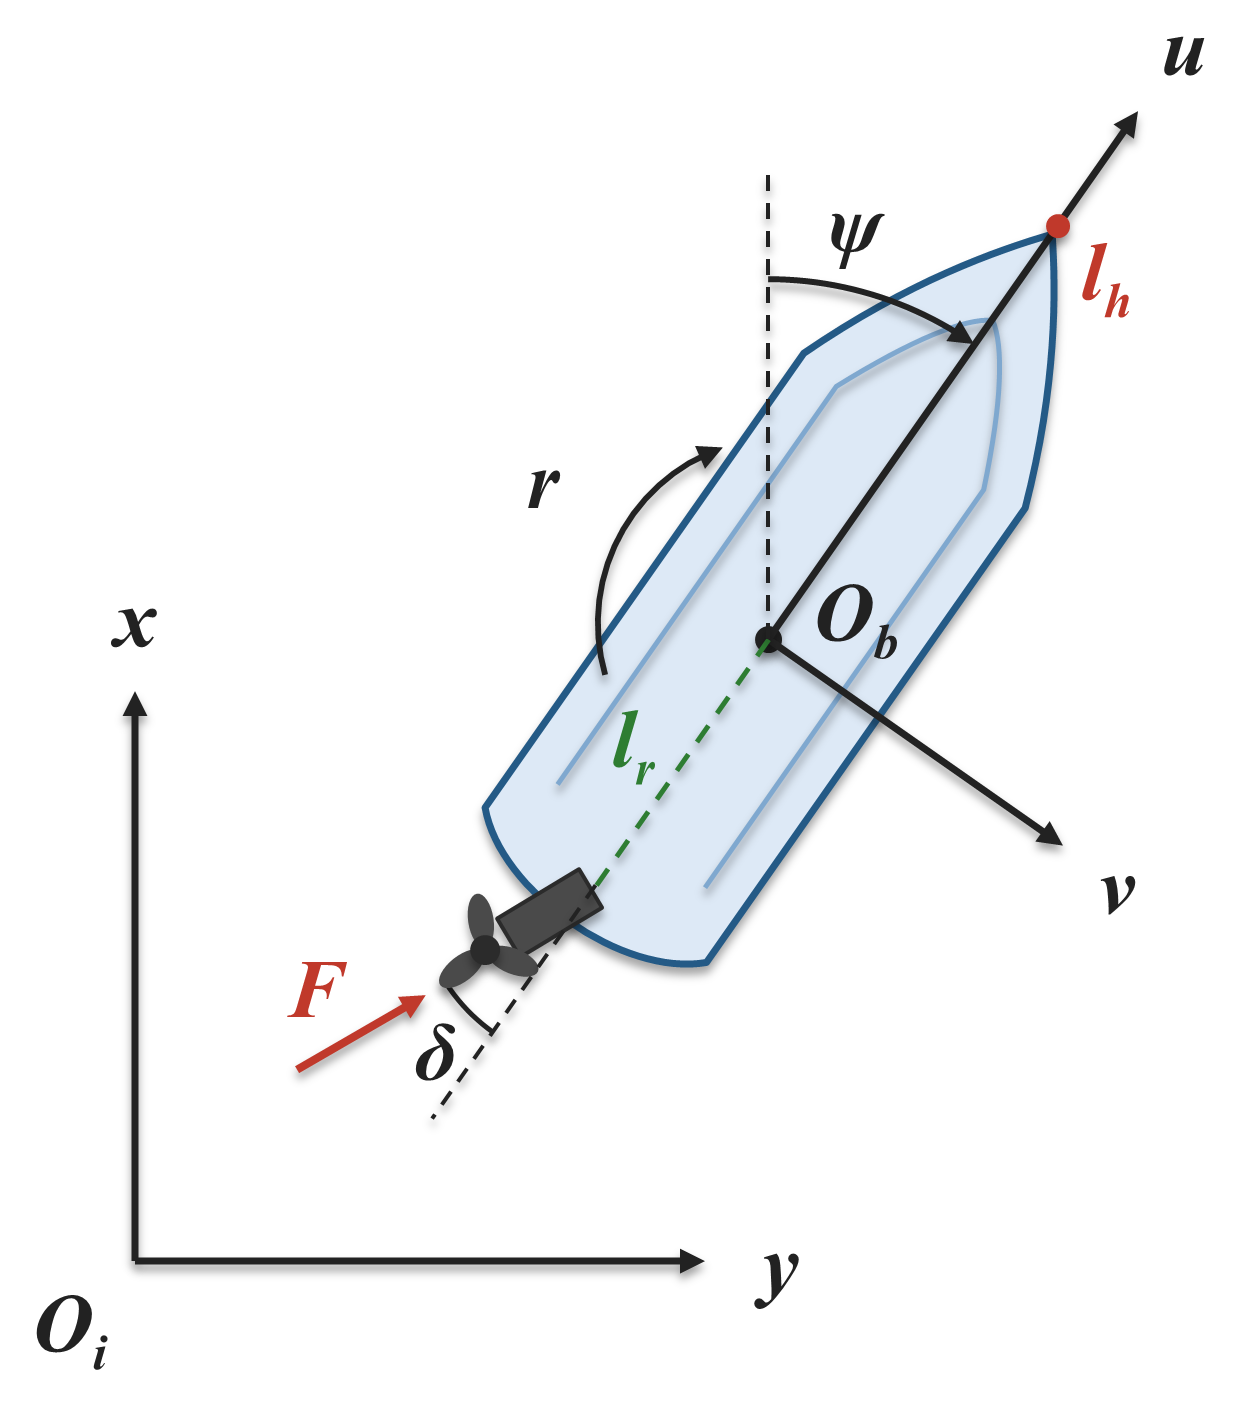
\includegraphics[width=0.6\linewidth]{fig/coordinate_frame}
\caption{Coordinate frames and actuator geometry of the USV.}
\label{fig_coordinate}
\end{figure}

The kinematics relate the body frame velocity $\nu = [u, v, r]^\top$ to the world frame pose $\eta = [x, y, \psi]^\top$ through the yaw rotation.
\begin{equation}\label{eq_kin}
\dot\eta = R(\psi)\,\nu,\qquad
R(\psi) = \begin{bmatrix} \cos\psi & -\sin\psi & 0 \\ \sin\psi & \cos\psi & 0 \\ 0 & 0 & 1 \end{bmatrix}.
\end{equation}
The kinetics are the identified maneuvering model of a model scale USV, written per unit mass and per unit inertia so that every coefficient is an acceleration.
\begin{equation}\label{eq_kinetics}
\begin{aligned}
\dot u &= X_u\,u + k_u F\cos\delta + w_u, \\
\dot v &= Y_{v|v|}\,|v|\,v + k_v F\sin\delta + w_v, \\
\dot r &= N_r\,r - k_r F\sin\delta + w_r,
\end{aligned}
\end{equation}
where $X_u$ is the linear surge damping, $Y_{v|v|}$ the quadratic sway damping, and $N_r$ the linear yaw damping. The single stern thruster of thrust $F$ deflected by the rudder angle $\delta$ drives all three axes through the gains $k_u$, $k_v$, and $k_r$, where $k_r$ lumps the moment arm $l_r$ of the thruster about the center of gravity marked in Fig.~\ref{fig_coordinate}. Sway is unactuated in the sense that it receives only the small side component of the deflected thrust. The vector $w = [w_u, w_v, w_r]^\top$ is the environmental disturbance expressed as body frame accelerations, bounded in the box
\begin{equation}\label{eq_wbox}
\mathcal{W} = \big\{\, w \,\big|\, |w_u|\le \bar w_u,\ |w_v|\le \bar w_v,\ |w_r|\le \bar w_r \,\big\},
\end{equation}
whose bound values are given in Table~\ref{tab_sim}. The identified coefficients are listed in Table~\ref{tab_params} in Section~\ref{sec_results}.

The rudder and thrust are bounded in amplitude, and their rates are bounded as well, so the admissible input sets are the following.
\begin{equation}\label{eq_amp}
\mathcal{U} = \big\{\, (\delta, F) \,\big|\, \delta_{\min}\le \delta\le \delta_{\max},\ F_{\min}\le F\le F_{\max} \,\big\},
\end{equation}
\begin{equation}\label{eq_rate}
\dot{\mathcal{U}} = \big\{\, (\dot\delta, \dot F) \,\big|\, \dot\delta_{\min}\le \dot\delta\le \dot\delta_{\max},\ \dot F_{\min}\le \dot F\le \dot F_{\max} \,\big\}.
\end{equation}


\begin{figure*}[t]
\centering
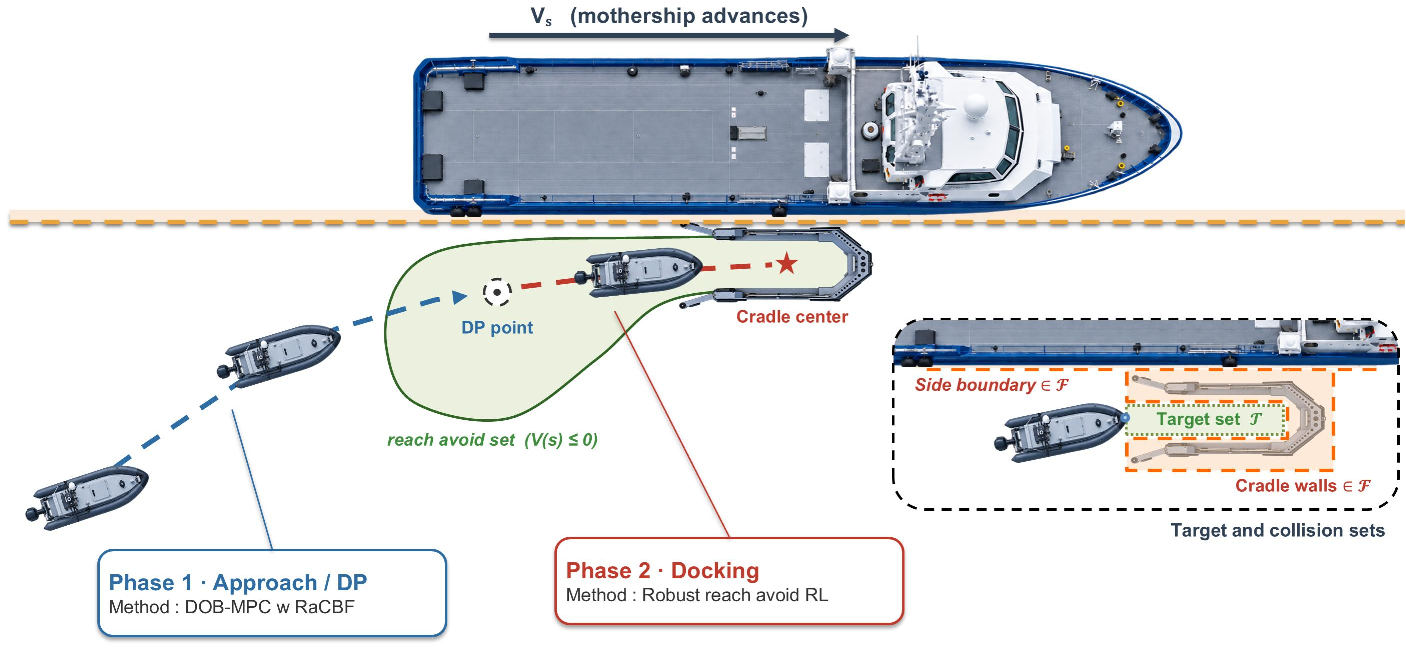
\includegraphics[width=\linewidth]{fig/recovery_scenario}
\caption{Top view of the recovery scenario. The mothership advances at the stream speed $V_s$ while the USV executes the two phase recovery, first approaching the dynamic positioning point and then docking from within the reach avoid set of the learned policy, and the zoom inset marks the target set inside the cradle and the surrounding collision set.}
\label{fig_scenario}
\end{figure*}


\section{Problem Formulation}\label{sec_problem}

The recovery task is illustrated in Fig.~\ref{fig_scenario}. An underactuated USV approaches from alongside the mothership and must enter the side cradle matched in position and heading, without striking the mothership hull or the cradle structure. Wind, wave, and current disturbance act on the vehicle throughout, and the cradle advances with the mothership at the stream speed $V_s$.

The problem is posed in a cradle fixed frame that advances with the mothership at $V_s$. Because the mothership is far larger and heavier than the USV, it maintains a steady heading and its motion is negligible over the recovery, and the crane stabilises the cradle against ship motion, so in this frame the cradle is nearly stationary. The state $s = [x_r, y_r, \psi_r, u, v, r, \delta, F]^\top \in \mathbb{R}^8$ collects the relative pose, the velocity, and the actuator states, and the control is the pair of actuator rates $a = [\dot\delta, \dot F]^\top$. The relative pose evolves in the cradle fixed frame as
\begin{equation}\label{eq_rel}
\begin{aligned}
\dot x_r &= u\cos\psi_r - v\sin\psi_r - V_s, \\
\dot y_r &= u\sin\psi_r + v\cos\psi_r,\qquad \dot\psi_r = r,
\end{aligned}
\end{equation}
with $(u, v, r)$ governed by \eqref{eq_kinetics}, the actuator states integrating the commanded rates, $\dot\delta = a_1$ and $\dot F = a_2$, with $a \in \dot{\mathcal{U}}$ and $(\delta, F)\in\mathcal{U}$, and the disturbance $w \in \mathcal{W}$ of \eqref{eq_wbox}. Two sets describe the outcome through scalar margin functions $\ell$ and $g$,
\begin{equation}\label{eq_margins}
\ell(s)\le 0 \iff s\in\mathcal{T},\qquad g(s)>0 \iff s\in\mathcal{F},
\end{equation}
evaluated at three points on the USV centerline, the center of gravity, the head point, a reference point at the bow a fixed distance forward of the center of gravity, and a stern point the same distance astern of it. The target set $\mathcal{T}$ requires the head point to enter the cradle pocket with the heading close to the cradle direction and a gentle relative velocity. The head point crosses the cradle mouth before the center of gravity does, and once it is inside the cradle, plain forward thrust alone draws the rest of the hull in after it. Reaching $\mathcal{T}$ with the head point, together with a heading aligned to the cradle, therefore already marks a docking that will complete, which is why the head point rather than the whole body is what must reach $\mathcal{T}$. The failure set $\mathcal{F}$ collects every state in which the head point, the center of gravity, or the stern point strikes the mothership hull or the head point strikes one of the three cradle arms, since the stern swings toward the mothership when the bow turns outboard, so all three points must stay clear. It also contains an approach wall that closes the outboard side of the cradle beyond its outer arm, so the pocket can be entered only through its mouth from astern. Both sets are marked in the zoom inset of Fig.~\ref{fig_scenario}, and the concrete geometry and numeric thresholds appear in Section~\ref{sec_results}.

The objective is to drive the USV so the head point reaches $\mathcal{T}$ while none of the three points ever enters $\mathcal{F}$, for every admissible disturbance, which defines a robust reach avoid problem.

\section{Control System Design}\label{sec_control}

\subsection{Recovery Framework}\label{sec_framework}
\begin{figure}[t]
\centering
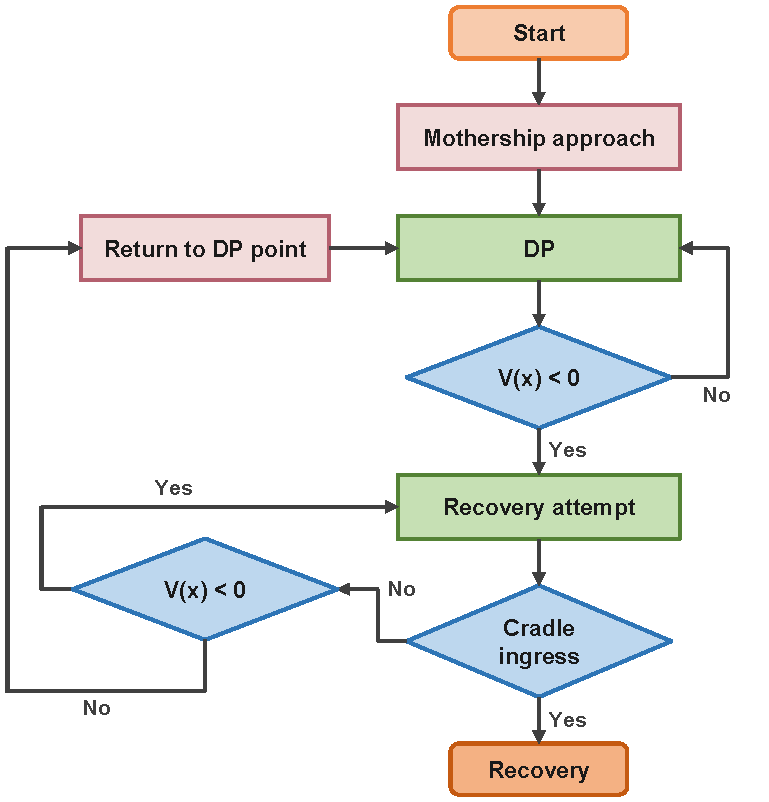
\includegraphics[width=0.9\linewidth]{fig/recovery_flowchart}
\caption{Recovery state machine. Phase 1 approaches the DP point and hands control to the Phase 2 reach avoid policy once the value crosses the handover threshold, and control falls back to Phase 1 if the state leaves the set before the cradle is entered.}
\label{fig_flowchart}
\end{figure}


The recovery runs in two phases, shown in Fig.~\ref{fig_scenario}. The reach avoid set must be computed over the whole region of states it is to cover, so relying on it for the far approach would be inefficient over such a large region, and far from the cradle there is relatively little to avoid. For these reasons Phase 1, the long approach and the dynamic positioning alongside the mothership, uses a disturbance observer based model predictive controller (DOB-MPC) with a robust adaptive control barrier function (RaCBF) \citep{park2026recovery}, in which the disturbance observer estimates the environmental disturbance, the DOB-MPC rejects it while respecting the actuator amplitude and rate limits over a horizon, and the RaCBF keeps the USV from colliding with the mothership. Near the cradle the situation is harsh, the cradle is narrow, the disturbance acts, and the USV is underactuated with actuation limits, so a guarantee of safe recovery is needed. Phase 2, the terminal docking, is therefore carried out by the robust reach avoid policy of Section~\ref{sec_rl}, whose certified set covers this terminal region.

The two phases are connected by a supervisor, whose state machine is shown in Fig.~\ref{fig_flowchart}. The Phase 2 policy of Section~\ref{sec_rl} carries the value function $V$ of the Hamilton Jacobi reach avoid problem, and the reach avoid set is where $V(s)<0$. From such a state the USV can reach the target and avoid the failure set under the worst case disturbance, and a state with $V(s)\ge 0$ lies outside the set. Phase 1 steers the USV toward the dynamic positioning (DP) point, which lies on the cradle centerline a short distance astern of the pocket mouth, and the supervisor evaluates $V$ along this approach. Control passes to the Phase 2 policy as soon as $V(s)\le\tau$, where $\tau$ is a small negative threshold (Table~\ref{tab_sim}) that leaves a margin against the approximation error of the learned value, and it returns to Phase 1 if $V(s)$ rises above zero before the cradle is entered, so a single scalar test governs both the transition and the abort. Once handed over, the funnel docking barrier of the Phase 1 controller is never activated. A disturbance larger than predicted can arrive suddenly, or a communication or mechanical fault can occur, and either can drive the state out of the reach avoid set during docking, so the sign test returns control to Phase 1 and the approach is retried.

\subsection{Robust Reach Avoid Reinforcement Learning}\label{sec_rl}
The terminal docking task posed above is a robust reach avoid problem. An underactuated USV with a single stern thruster and rudder must enter a cradle that moves with the mothership while a bounded environmental disturbance acts on the hull, and we solve it with Hamilton Jacobi reachability \citep{mitchell2005time, bansal2017hamilton, lygeros2004reachability}. The reachability value function assigns to each state a single signed scalar, the best reach avoid outcome achievable from that state over the horizon under the worst case disturbance, so it behaves like a signed margin to the boundary of the recoverable set. The value is negative inside the set and positive outside. It is most negative deep inside, where the state is recovered with the widest margin, it approaches zero at the boundary, and outside the set it is positive by the amount the best control still fails to reach the cradle without touching the failure set. This margin is a value margin rather than a literal Euclidean distance, since it stays negative throughout the interior. The state $s$, the target set $\mathcal{T}$, the failure set $\mathcal{F}$, and the margins $\ell$ and $g$ were defined in Section~\ref{sec_problem}. As established there, the target margin is read at the head point, the avoid margin checks the head point against the cradle arms and the approach wall and the head point, the center of gravity, and the stern point against the mothership side, and the value and its zero sublevel set are drawn over the head point position throughout.

The control minimizes the reach avoid outcome while the worst case disturbance maximizes it, a two player differential game in the sense of Margellos and Lygeros \citep{margellos2011hamilton, fisac2015reach, hsu2021safety}. Writing $\xi^{a,w}_s(\cdot)$ for the trajectory from $s$ under control $a$ and disturbance $w$, with $t$ and $\kappa$ times along it, the value is
\begin{equation}\label{eq_payoff}
V(s) = \inf_{a}\ \sup_{w}\ \min_{t\ge 0}\, \max\Big\{ \ell\big(\xi^{a,w}_s(t)\big),\ \max_{\kappa\in[0,t]} g\big(\xi^{a,w}_s(\kappa)\big) \Big\}.
\end{equation}
The value is at most zero exactly on the robust reach avoid set $\mathrm{RA}(\mathcal{T},\mathcal{F})$, the states from which some control drives the head point into $\mathcal{T}$ and keeps the reference points clear of $\mathcal{F}$ against every admissible disturbance, that is $V(s)\le 0 \iff s\in\mathrm{RA}(\mathcal{T},\mathcal{F})$. Dynamic programming turns \eqref{eq_payoff} into the robust reach avoid Bellman equation \citep{hsu2021safety}. With $s'_{a,w}$ the next state under $a$ and $w$ it reads
\begin{equation}\label{eq_rabe}
V(s) = \max\Big\{ g(s),\ \min\big\{ \ell(s),\ \inf_{a}\ \sup_{w}\ V(s'_{a,w}) \big\} \Big\}.
\end{equation}
Grid based dynamic programming solves \eqref{eq_rabe} in the classical setting but scales exponentially with the state dimension and cannot reach the eight dimensional state of Section~\ref{sec_model}, which motivates a learning method. Discounting by $\gamma\in[0,1)$ makes the backup a contraction \citep{fisac2019bridging, hsu2021safety} and yields the robust discounted reach avoid Bellman equation, whose operator we denote $\mathcal{B}_\gamma$,
\begin{equation}\label{eq_drabe}
\begin{aligned}
V_\gamma(s) = {}& (1-\gamma)\max\{\ell(s), g(s)\} \\
&+ \gamma\,\max\Big\{ g(s),\ \min\big\{ \ell(s),\ \inf_{a}\ \sup_{w}\ V_\gamma(s'_{a,w}) \big\} \Big\}.
\end{aligned}
\end{equation}
We do not claim this backup as our own. The robust discounted backup is the reach avoid game counterpart of the discounted reach avoid backup of \citet{hsu2021safety} and \citet{fisac2019bridging}, and related robust and reachability constrained formulations appear in \citet{li2023robust, hsu2023isaacs, yu2022reachability}. Our contribution is not the backup but learning its value and a deployable robust policy for cradle recovery of an underactuated USV. Two guarantees carry over from the undisturbed case and are proved in Appendix~\ref{app_proofs}.
\begin{proposition}\label{prop_contraction}
For every $\gamma\in[0,1)$ the operator $\mathcal{B}_\gamma$ is a contraction under the supremum norm, so \eqref{eq_drabe} has a unique fixed point $V_\gamma$.
\end{proposition}
\begin{theorem}\label{thm_underapprox}
For discount factors $0\le\gamma_1\le\gamma_2<1$ the induced sets satisfy $\mathrm{RA}_{\gamma_1}\subseteq\mathrm{RA}_{\gamma_2}\subseteq\mathrm{RA}(\mathcal{T},\mathcal{F})$, where $\mathrm{RA}_{\gamma}=\{s\,|\,V_\gamma(s)\le 0\}$, and $\mathrm{RA}_{\gamma}$ converges to $\mathrm{RA}(\mathcal{T},\mathcal{F})$ in the Hausdorff distance as $\gamma\to 1$.
\end{theorem}
The fixed point is therefore a conservative under approximation of the true robust reach avoid set. A state the value declares recoverable is recoverable under the worst case disturbance up to function approximation error, which is what makes the sign of $V$ a sound certificate for the handoff of Section~\ref{sec_framework}.

The practical algorithm represents the value with twin critics $Q_1, Q_2$ and two actors.
\begin{equation}\label{eq_value}
V(s) = \min\big(Q_1, Q_2\big)\big(s, \pi(s), \mu(s)\big),
\end{equation}
where $\pi$ is the protagonist actor that minimizes the value and $\mu$ is the adversary actor that maximizes it. The critics regress onto an $N$ step target computed on subtrajectories drawn from the replay buffer and unrolled backward from a bootstrapped tail.
\begin{equation}
y_N = \min\big(Q_1^{-}, Q_2^{-}\big)\big(s_{t+N}, \pi(s_{t+N}), \mu(s_{t+N})\big),
\end{equation}
\begin{equation}
\begin{aligned}
y_k = {}& (1-\gamma)\max\big(g_k, \ell_k\big) \\
&+ \gamma\max\Big(g_k, \min\big(\ell_k, y_{k+1}\big)\Big),\ k = N-1, \dots, 0,
\end{aligned}
\end{equation}
where $Q_1^{-}, Q_2^{-}$ are target networks and $\ell_k, g_k$ are the reach and avoid payoffs along the stored subtrajectory. Setting $N=1$ recovers \eqref{eq_drabe} in a single step, while larger $N$ folds the reach and avoid information of $N$ consecutive payoffs into one regression target and propagates it backward correspondingly faster. The discount $\gamma$ is set close to one so that the induced set stays a tight under approximation of the true reach avoid set. % CHECK: gamma = 0.999 and N = 5 are carried over from the earlier ris_ms runs. The s140w_conv.pt checkpoint does not store them, confirm against the ris_surge training config.
In the trained policy the discount is $\gamma=0.999$, the target spans $N=5$ steps, the control period is 0.25 s, and the adversary plays within the disturbance bound $\mathcal{W}$ of \eqref{eq_wbox}.

The implementation follows the TD3 recipe. The minimum of the twin critics is used everywhere the value appears, which limits the overestimation that would otherwise inflate the reachable set, target networks are updated by soft Polyak averaging, and both actors are updated at a reduced frequency relative to the critics. The delayed updates proved necessary, since with synchronous updates the actor diverged near the corridor edge where the reach and avoid branches of the backup exchange dominance. Two further training measures were essential. First, the adversary is introduced through a staged disturbance ramp that starts at a zero bound and grows in stages to the full box, so the protagonist first learns a nominal docking maneuver and then hardens it, whereas training against the full adversary from the start collapsed to overly conservative behavior. Second, both the mothership side wall and the approach wall are kept in the avoid margin during training. Without the side wall the learned value marked parts of the mothership interior as reachable, and the approach wall keeps the learned set from claiming entries around the outer arm, so every certified state enters the pocket from astern. The policy was trained for $6\times10^{4}$ updates, and the staged ramp ends at the full bound $\mathcal{W}$.



\section{Simulation Result}\label{sec_results}

The proposed framework was validated in numerical simulation of the model scale USV of Section~\ref{sec_model} against the Phase 1 controller carried through the entire docking, over a Monte Carlo campaign of physically generated sea scenarios. The model coefficients and actuator limits are collected in Table~\ref{tab_params}, the docking geometry in Table~\ref{tab_set} and Fig.~\ref{fig_setgeom}, and the simulation and training settings in Table~\ref{tab_sim}. Every controller faces the identical scenarios, initial states, and seas, so the comparison is paired and only the control law differs.

The reach and avoid conditions are evaluated at the head point, at position $(x_h, y_h)$ a distance $l_h$ forward of the center of gravity, because the bow crosses the cradle mouth first. The target margin takes the box form
\begin{equation}\label{eq_reach}
\begin{aligned}
\ell(s) = \max\big(&|x_h|-C_X,\ |y_h|-C_Y,\ |\psi_r|-\Theta, \\
&|\dot x_r|-U_d,\ |\dot y_r|-U_d\big),
\end{aligned}
\end{equation}
so the head point must lie inside the pocket, the heading within $\Theta$ of the cradle, and the cradle relative velocity within the docking gate $U_d$ on both axes, and a state that meets the gate enters nearly at rest relative to the cradle. The avoid margin is the pointwise maximum over the obstacles,
\begin{equation}\label{eq_avoid}
g(s) = \max_{i}\, g_i(s),
\end{equation}
where each $g_i$ is the signed margin of one obstacle, positive when it is violated, so $g$ takes the value of the most violated one. The obstacles are the three cradle arms checked at the head point, the mothership side boundary checked at the head point, the center of gravity, and the stern point, and the approach wall checked at the head point. The approach wall is a training device. In the evaluation a failure is counted only for physical contact with a cradle arm or the mothership side, and the clearance reported below is the distance to the nearest physical obstacle, the negative of the avoid margin, positive while clear and zero at contact.

\begin{figure}[t]
\centering
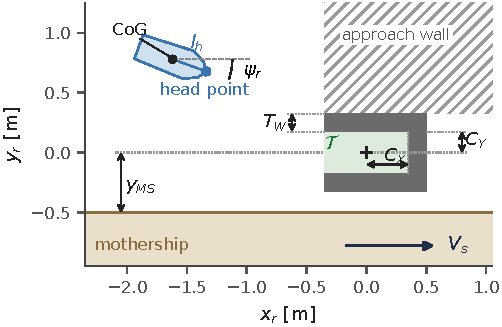
\includegraphics[width=0.95\linewidth]{fig/set_geometry}
\caption{Geometry of the docking target and the collision set in the cradle fixed frame, with the variables of Table~\ref{tab_set}. The pocket half sizes $C_X$ and $C_Y$, the arm thickness $T_W$, the mothership side $y_{MS}$, the head point offset $l_h$, the relative heading $\psi_r$, and the stream speed $V_s$ are marked, the hatched approach wall closes the outboard side beyond the outer arm, and the target set $\mathcal{T}$ is shaded inside the pocket.}
\label{fig_setgeom}
\end{figure}



\begin{figure*}[t]
  \centering
  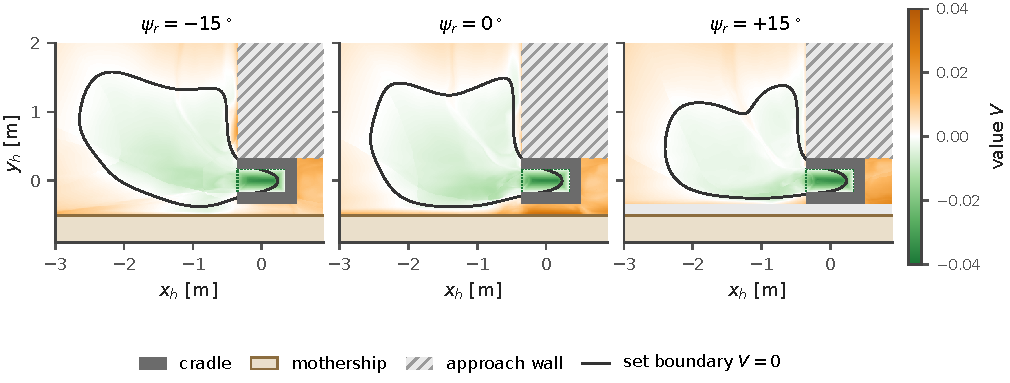
\includegraphics[width=\linewidth]{fig/reach_avoid_set}
  \caption{Learned robust reach avoid set at three relative headings on the nominal slice with zero cradle relative velocity and trim thrust, drawn over the head point position. The value $V$ is shaded, the set boundary $V=0$ is solid, and the cradle, the mothership, and the hatched approach wall are drawn.}
  \label{fig_set}
\end{figure*}

\begin{figure*}[t]
  \centering
  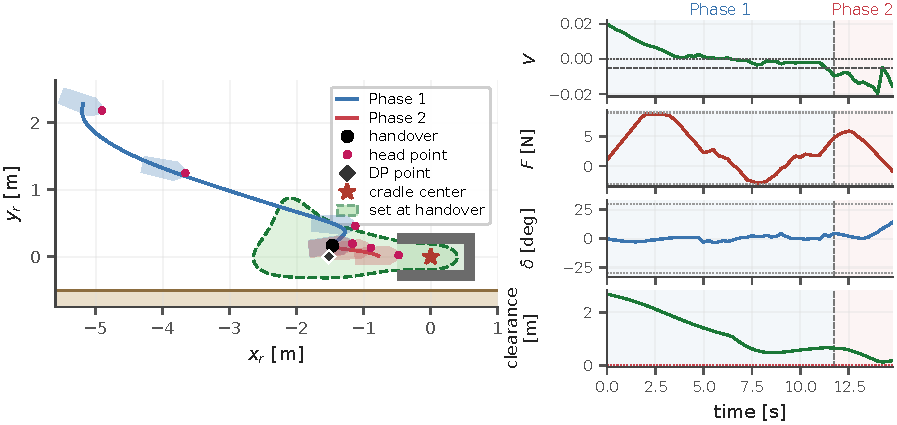
\includegraphics[width=0.9\linewidth]{fig/rep_run}
  \caption{Representative recovery of the proposed framework in the cradle fixed frame. The left panel draws the vessel outlines along the path, Phase 1 in blue and Phase 2 in red, with the head points, the handover point, the DP point, the cradle center, and the learned set evaluated at the handover state. The right panels show the value $V$, the thrust $F$, the rudder angle $\delta$, and the clearance against time, with the two phases shaded and the handover marked by the vertical dashed line.}
  \label{fig_representative}
\end{figure*}

The disturbance $w$ collects the wind and wave loads of the model of \citet{fossen2011handbook}, a mean wind force, a slowly varying second order wave drift, and a first order wave force, resolved into the body surge, sway, and yaw axes and clipped into $\mathcal{W}$. The bound is fixed in advance, and both the training adversary and the evaluation seas act within it. In each sea scenario the wind and waves share a common bearing drawn within a sector around the bow, a wind to wave ratio is drawn, and the significant wave height is then set close to the largest value whose peak load still fits inside $\mathcal{W}$, so every scenario loads the vehicle near the edge of the bound, and sway is the channel that binds in almost every scenario. The USV starts astern and outboard of the cradle, heading toward the cradle line and moving with the stream, within the ranges of Table~\ref{tab_sim}.

The baseline is the Phase 1 DOB-MPC with RaCBF \citep{park2026recovery} carried through the entire docking, in which a funnel docking barrier becomes active in its docking phase. Two docking barrier gains are compared, a permissive gain (1) and a conservative gain (2), the two ends of the gain trade off for the same controller, listed in Table~\ref{tab_sim}. Both use the same fixed robust margin, and the barrier also checks the stern, so both methods share the collision model. Recovery outcome, docking time, and minimum clearance are summarized in Fig.~\ref{fig_montecarlo}, sample paths in Fig.~\ref{fig_trajectories}, and the per call computation time in Table~\ref{tab_compute}.

\begin{figure*}[t]
  \centering
  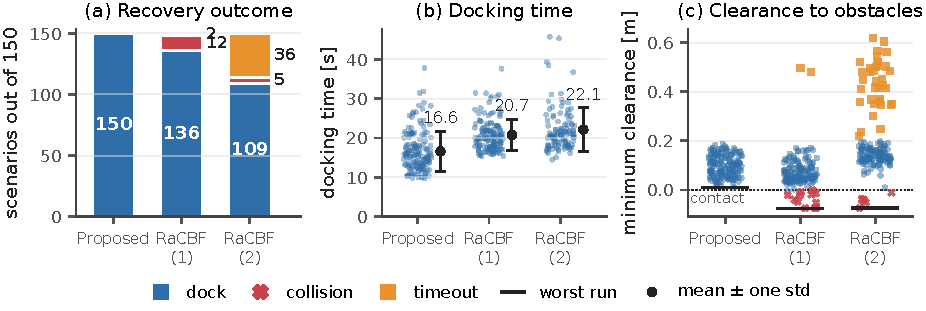
\includegraphics[width=\linewidth]{fig/montecarlo_summary}
  \caption{Monte Carlo summary over the sea scenarios of Table~\ref{tab_sim}. (a) Recovery outcome counted as docks, collisions, and timeouts. (b) Docking time over the docked runs, each run a dot with the mean and one standard deviation. (c) Minimum clearance of every run coloured by outcome, with the worst run per controller as a bar and the contact line at zero. The two docking barrier gains of the DOB-MPC with RaCBF baseline are labelled (1) and (2).}
  \label{fig_montecarlo}
\end{figure*}

\begin{figure*}[t]
  \centering
  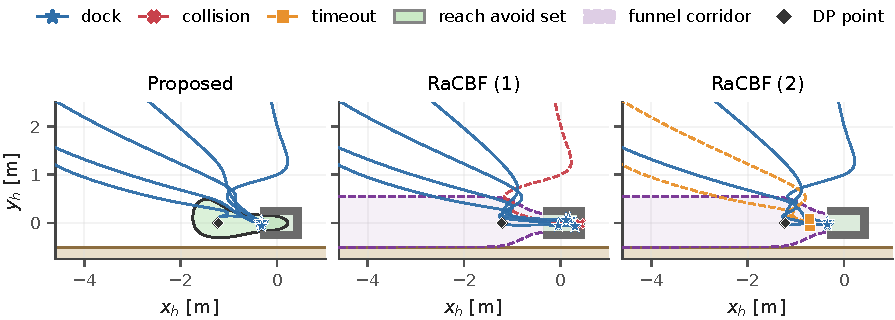
\includegraphics[width=\linewidth]{fig/trajectories_montecarlo}
  \caption{Head point paths of the same five sea scenarios under each controller. Docked runs are drawn solid and end with a star, collisions dashed with a cross, and timeouts dashed with a square, and the DP point is marked with a diamond. The proposed panel shades the reach avoid set at the DP point, whereas the baseline panels shade the funnel corridor of the DOB-MPC with RaCBF.}
  \label{fig_trajectories}
\end{figure*}

The learned robust reach avoid set is shown in Fig.~\ref{fig_set} on the nominal slice at three relative headings, with zero cradle relative velocity and trim thrust, drawn over the head point position. The set is nearly as large with the bow turned inboard as when the USV is aligned with the cradle, and smaller when the bow turns outboard toward the approach wall. It stays clear of the mothership side and of the approach wall and reaches into the pocket. The handover of Section~\ref{sec_framework} uses the stricter level $\tau$ inside this set. Because the discounted value under approximates the true set, the shaded region is a conservative estimate.

A representative recovery is shown in Fig.~\ref{fig_representative}, a scenario that starts far astern and outboard and that the conservative baseline fails to complete. In the left panel Phase 1 carries the USV toward the DP point, the value crosses the handover threshold, and the Phase 2 policy turns the hull into the pocket from inside the learned set evaluated at the handover state. In the right panels the value falls through zero during the Phase 1 approach and crosses $\tau$ at the handover. Thrust rises close to its upper limit early in the approach, is then reduced and reaches reverse around the handover, after which the policy raises it briefly and eases it off so the hull enters slowly, while the rudder stays well inside its limits. The clearance decreases toward the cradle and stays positive throughout, so the recovery is safe and admissible at once.

Aggregate behavior over the scenario set appears in Fig.~\ref{fig_montecarlo}. In panel (a) the proposed method docks in every scenario, RaCBF (1) loses a few runs to collisions with the cradle and has no timeouts, and RaCBF (2) has no collisions but several timeouts. In the RaCBF (1) collisions the hull reaches the back of the pocket before slowing to the docking gate and strikes the back of the cradle, and in the RaCBF (2) timeouts the stronger barrier holds the hull just astern of the pocket mouth and it never enters. The barrier gain therefore trades one failure for the other, soft action admits contact while conservative action blocks entry, whereas the proposed policy has no barrier gain to tune, and the supervisor handed over in every scenario. Panel (b) shows that the proposed method docks fastest on average over the docked runs, with a spread comparable to RaCBF (1) and far tighter than RaCBF (2), which is the slowest with a long tail. Panel (c) shows the minimum clearance of every run. The proposed method and RaCBF (2) keep positive clearance in every run while RaCBF (1) makes contact. The runs of the proposed method sit in a narrow positive band because every run enters the pocket, whereas RaCBF (2) holds a larger clearance because its stronger barrier keeps the hull off and its timeouts never enter.

The three panels of Fig.~\ref{fig_trajectories} overlay the head point paths of the same five scenarios under each controller, chosen so that every baseline failure mode appears. The proposed paths all converge into the set and dock at the pocket mouth. RaCBF (1) docks every run except one, whose head point stays outside the funnel corridor on the final approach, crosses its boundary only at the pocket mouth, and then strikes the back of the cradle, and RaCBF (2) docks some and stalls just astern of the mouth in the others.

The computation times in Table~\ref{tab_compute} complete the comparison, each controller timed alone on an otherwise idle machine. The Phase 2 policy is a single network evaluation with no online optimization, far cheaper than one DOB-MPC solve, and its worst case sits well inside the control period, whereas the baselines keep solving the MPC throughout their docking.

\begin{table}[t]
  \centering
  \caption{Per call computation time of each controller over the sea scenarios, measured alone on an otherwise idle machine. For the proposed method the Phase 2 row is the reach avoid policy, a single network evaluation.}
  \label{tab_compute}
  \begin{tabular}{lcc}
    \hline
    Controller and phase & Mean [ms] & Max [ms] \\
    \hline
    Proposed, Phase 1 DOB-MPC with RaCBF & 20.0 & 53.2 \\
    \textbf{Proposed, Phase 2 reach avoid policy} & \textbf{0.8} & \textbf{1.7} \\
    RaCBF (1), docking phase & 18.6 & 22.1 \\
    RaCBF (2), docking phase & 19.5 & 26.9 \\
    \hline
  \end{tabular}
\end{table}

\begin{table}[t]
\centering
\renewcommand{\arraystretch}{1.2}
\caption{Actuator limits and identified coefficients of the model scale USV.}
\label{tab_params}
\resizebox{\linewidth}{!}{%
\begin{tabular}{cc|cc}
\hline
\multicolumn{2}{c|}{\textbf{Actuator Limits}} & \multicolumn{2}{c}{\textbf{Model Coefficients}} \\ \hline
\textbf{Parameter} & \textbf{Value [Unit]} & \textbf{Parameter} & \textbf{Value} \\ \hline
$\delta$     & $\pm 30$ [deg]   & $X_u$       & $-0.1985$ \\
$\dot\delta$ & $\pm 15$ [deg/s] & $Y_{v|v|}$  & $-0.13$   \\
$F$          & $[-3,\ 9]$ [N]   & $N_r$       & $-0.1$    \\
$\dot F$     & $\pm 4$ [N/s]    & $k_u$       & $0.0594$  \\
             &                  & $k_v$       & $0.007$   \\
             &                  & $k_r$       & $0.157$   \\
\hline
\end{tabular}}
\end{table}

\begin{table}[t]
\centering
\renewcommand{\arraystretch}{1.2}
\caption{Parameters of the docking target and the collision set.}
\label{tab_set}
\begin{tabular}{lc}
\hline
\textbf{Parameter} & \textbf{Value [Unit]} \\ \hline
Head point offset ($l_h$)         & 0.3 [m]   \\
Pocket half length ($C_X$)        & 0.35 [m]  \\
Pocket half width ($C_Y$)         & 0.175 [m] \\
Arm thickness ($T_W$)             & 0.15 [m]  \\
Mothership side ($y_{MS}$)        & $-0.5$ [m] \\
Approach wall ($y_A$)             & 0.325 [m] \\
Heading tolerance ($\Theta$)      & 30 [deg]  \\
Docking gate ($U_d$)              & 0.24 [m/s] \\
\hline
\end{tabular}
\end{table}

\begin{table}
\centering
\renewcommand{\arraystretch}{1.2}
\caption{Simulation, scenario, and training settings.}
\label{tab_sim}
\begin{tabular}{lc}
\hline
\textbf{Parameter} & \textbf{Value [Unit]} \\ \hline
Stream speed ($V_s$)                          & 0.5 [m/s] \\
Control period                                & 0.25 [s] \\
Plant integration step                        & 0.01 [s] \\
Disturbance bound ($\bar w_u$, $\bar w_v$)    & 0.1059, 0.01275 [m/s$^2$] \\
Disturbance bound ($\bar w_r$)                & 0.01785 [rad/s$^2$] \\
DP point ($x_r$, $y_r$)                       & $(-1.52,\ 0)$ [m] \\
Handover threshold ($\tau$)                   & $-0.005$ \\
Initial position $x_r$                        & $[-6.5,\ -0.5]$ [m] \\
Initial position $y_r$                        & $[2.0,\ 6.0]$ [m] \\
Initial heading ($\psi_r$)                    & $-20$ [deg] \\
Sea direction sector                          & $\pm 70$ [deg] \\
Sea scenarios                                 & 100 \\
Episode horizon                               & 120 [s] \\
Training updates                              & $6\times 10^{4}$ \\
RaCBF docking gains (1)                       & 4.0, 0.7 \\
RaCBF docking gains (2)                       & 0.55, 0.55 \\
\hline
\end{tabular}
\end{table}

\section{Conclusion}\label{sec_conclusion}

This paper formulated the docking phase of USV cradle recovery as a robust discounted reach avoid game whose fixed point under approximates the true reach avoid set and converges to it as the discount tends to one, and embedded the learned value and policy in a two phase framework in which set membership decides both the handover from the approach controller and the fallback out of the docking phase. In Monte Carlo simulation of a model scale USV over physically generated seas that load the vehicle near its disturbance bound, the framework docked in every scenario without contact and faster on average, whereas the barrier based controller struck the cradle or stalled depending on its gain, and the docking policy runs in a small fraction of the control period. The certificate is only as good as the learned value, and the method has not yet been tested on hardware at sea, so future work will pursue verified error bounds on the learned set and experimental recovery campaigns.

\begin{appendices}
\section{Proofs}\label{app_proofs}
\begin{proof}[Proof of Proposition~\ref{prop_contraction}]
Write $\mathcal{B}_\gamma V(s) = (1-\gamma)\max\{\ell(s),g(s)\} + \gamma\,\mathcal{H}[V](s)$, where $\mathcal{H}[V](s) = \max\{g(s),\ \min\{\ell(s),\ \inf_{a}\sup_{w} V(s'_{a,w})\}\}$. The first term does not depend on $V$. For bounded functions $V$ and $V'$, taking an infimum over $a$ and a supremum over $w$ of quantities that differ pointwise by at most $\|V-V'\|_\infty$ changes the result by at most $\|V-V'\|_\infty$, and the maps $x\mapsto\min\{\ell(s),x\}$ and $x\mapsto\max\{g(s),x\}$ are nonexpansive. Composing these nonexpansive operations gives $|\mathcal{H}[V](s)-\mathcal{H}[V'](s)|\le\|V-V'\|_\infty$ for every $s$, so $\|\mathcal{B}_\gamma V-\mathcal{B}_\gamma V'\|_\infty\le\gamma\,\|V-V'\|_\infty$. Hence $\mathcal{B}_\gamma$ is a contraction of modulus $\gamma$ on the bounded functions under the supremum norm, and the Banach fixed point theorem yields a unique fixed point $V_\gamma$. The argument follows the discounted reach avoid backup of \citet{hsu2021safety} and \citet{fisac2019bridging}, with the single control infimum replaced by the game value $\inf_{a}\sup_{w}$.
\end{proof}
\begin{proof}[Proof of Theorem~\ref{thm_underapprox}]
By Proposition~\ref{prop_contraction} each $V_\gamma$ is well defined. Discounting is conservative, so $V_\gamma$ upper bounds the undiscounted value $V$ of \eqref{eq_rabe}, which gives $\mathrm{RA}_\gamma=\{V_\gamma\le 0\}\subseteq\{V\le 0\}=\mathrm{RA}(\mathcal{T},\mathcal{F})$. The induced sets are nested in the discount, $\mathrm{RA}_{\gamma_1}\subseteq\mathrm{RA}_{\gamma_2}$ for $\gamma_1\le\gamma_2$, and they grow to $\mathrm{RA}(\mathcal{T},\mathcal{F})$ in the Hausdorff distance as $\gamma\to 1$. These monotonicity and convergence properties are the reach avoid game counterpart of the discounted analysis of \citet{fisac2019bridging} and \citet{hsu2021safety}, which is unchanged when the single control operator is replaced by the game value $\inf_{a}\sup_{w}$, and we refer to those works for the full limiting argument.
\end{proof}
\end{appendices}


\bibliographystyle{agsm}
\bibliography{bib}

\end{document}
